\documentclass[border=10pt]{standalone}
%%%<
\usepackage{verbatim}
%%%>
\usepackage{pgfplots}
\usepackage{pgfplotstable}
\usetikzlibrary{patterns}
\pgfplotstableset{fixed zerofill,precision=3}
\pgfplotsset{width=7cm,compat=1.8}
\begin{comment}
:Title: Bar plot
:Tags: 2D;Bar plots;Manual
:Author: Christian Feuersänger
:Slug: bar-plot

Bar plots place horizontal or vertical bars at coordinates. Multiple bar plots
in one axis can be stacked on top of each other or aligned next to each other.

The code is from the PGFPlots 1.10 manual: "4.5.4 Bar Plots".
\end{comment}
\begin{document}
	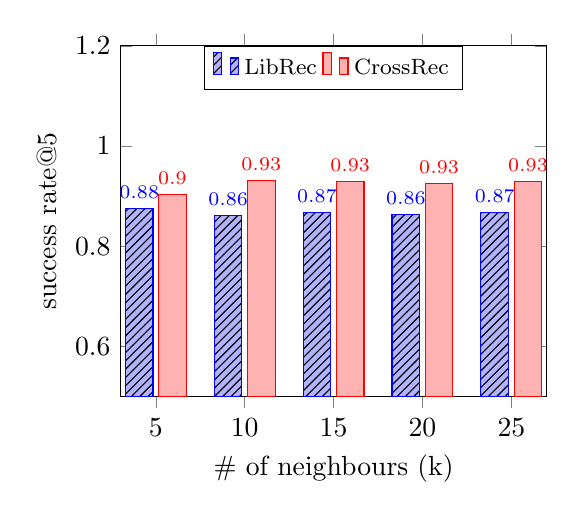
\begin{tikzpicture}
	\begin{axis}[
	ybar,
	%enlargelimits=0.15,
		legend style={at={(0.5,1)},	anchor=north,legend columns=-1,font=\footnotesize},
	xlabel={\# of neighbours (k)},
	ylabel={success rate@5},
	symbolic x coords={5,10,15,20,25},
	xtick=data,
	nodes near coords,
	nodes near coords align={vertical},
	every node near coord/.append style={font=\scriptsize},
	ymin=0.5,ymax=1.2,
	]
	\addplot +[postaction={pattern=north east lines}] coordinates {(5,0.876) (10,0.862) (15,0.868) (20,0.863) (25,0.868)};
	\addplot coordinates {(5,0.903) (10,0.931) (15,0.929) (20,0.926) (25,0.929)};
	\legend{LibRec,CrossRec}
	\end{axis}
	\end{tikzpicture}
\end{document}
